\documentclass[twocolumn]{llncs}
\setlength{\columnsep}{15pt}
\makeatletter
\renewcommand{\section}{\@startsection{section}{1}{\z@}%
  {-2.0ex plus -0.5ex minus -.2ex}%
  {1.0ex plus 0.2ex}%
  {\centering\normalfont\normalsize\bfseries}}
\makeatother

\makeatletter
\renewcommand{\subsection}{\@startsection{subsection}{2}{\z@}%
  {-0.3\baselineskip}  % khoảng cách TRÊN (mặc định ~2.0)
  {0.3\baselineskip}   % khoảng cách DƯỚI (mặc định ~1.0)
  {\normalfont\normalsize\bfseries}}
\makeatother

\usepackage{hyperref}
\usepackage{enumitem}
\usepackage[justification=centering]{caption}
\usepackage{amsmath}
\usepackage{amsfonts}
\usepackage{booktabs}
\usepackage{graphicx}
\usepackage[T1]{fontenc}
\usepackage{float}
\usepackage[a4paper, left=2cm, right=2cm, top=3cm, bottom=3cm]{geometry}

\renewcommand{\thesection}{\Roman{section}}        % I, II, III, ...
\renewcommand{\thesubsection}{\Roman{section}.\Alph{subsection}} % I.A, I.B, ...
\renewcommand{\thesubsection}{\Alph{subsection}}


\begin{document}
% ==============================================================
% =====================    TITLE   =============================
% ==============================================================
\twocolumn[{
\title{Time Series Analysis for Tesla Stock Prediction Using Machine Learning}

% ==============================================================
% =====================    AUTHOR   ============================
% ==============================================================

\author{Nguyen Tien Dat\inst{1} 
\and Vo Quoc Huy\inst{2}
\and Bui Minh Duy\inst{3}
\and Cao My Duyen\inst{4} 
\and Nguyen Thien Kim\inst{5}}

\institute{
University of Information Technology,
\email{22520226@gm.uit.edu.vn}
\and
University of Information Technology,
\email{22520586@gm.uit.edu.vn}
\and
University of Information Technology,
\email{22520311@gm.uit.edu.vn}
\and
University of Information Technology,
\email{22520347@gm.uit.edu.vn}
\and
University of Information Technology,
\email{22520729@gm.uit.edu.vn}
}

% ==============================================================
% =====================    ABSTRACT   ==========================
% ==============================================================
\maketitle

\begin{abstract}
Machine learning and deep learning techniques are renowned for playing a pivotal role in Business Analytics by leveraging time-series datasets to provide businesses with insights that assist in decision-making, improve performance, and optimize processes. With the rapid and diverse development of algorithms, there arises a critical need to scrutinize their efficacy within specific domains. This paper addresses this need by utilizing and evaluating six distinct algorithms - ARIMA, SVR, RNN, ResNet, ResNetLSTM - for forecasting the stock price of Tesla Inc. based on historical daily stock price records. The objective of this study is to analyze and predict the trajectory of Tesla's stock prices, considering recent market challenges such as intensified competition in the electric vehicle sector and broader political uncertainties affecting the financial markets. The study conducts a comparative analysis of the predictive capabilities of these algorithms and presents a detailed methodology explaining the selection and application of each model. Based on the analyses, the study highlights the strengths and limitations of each approach. Through systematic evaluation and comparison, the paper aims to enhance the understanding of the suitability and competence of these algorithms for stock price analysis and prediction in the context of Tesla’s volatile market environment.

\keywords{Tesla Stock Prediction \and Machine Learning \and Deep Learning \and Time-Series Forecasting \and Linear Regression \and ARIMA \and ResNet \and ResNetLSTM \and Stock Price Analysis}
\end{abstract}
}]


% ==============================================================
% =====================       DATA       =======================
% ==============================================================
\section{MATERIALS}
\subsection{Dataset}
In this study, we scrutinize the historical stock price data for Tesla Inc. (TSLA), sources directly from the Yahoo Finance API. The dataset includes daily information spanning from June 29th, 2010 to May 23th 2025, covering over 3,000 trading days. Each record includes variables that provide important insights and data for the study, specifically as follows:
\renewcommand{\labelitemi}{\textbullet} 
\begin{itemize}[itemsep=1em]
    \item Date: The specific day the stock price was recorded.
    \item Open: Tesla's stock price at the start of the trading day.
    \item High: The highest price Tesla's stock reached during that day's trading.
    \item Low: The lowest price Tesla's stock dropped to during that day's trading.
    \item Close: Tesla's stock price when the market closed for the day.
    \item Adj Close (Adjusted Close): The closing price, adjusted to account for significant corporate actions like dividends or stock splits.
    \item Volume: The total number of Tesla shares that changed hands on that particular day.
\end{itemize}
This data reflects the daily fluctuations in Tesla's stock price and is used to train models that forecast future price trends.
%
\subsection{Descriptive Statistics}
\begin{figure}[H]
    \centering
    \begin{minipage}[b]{0.48\linewidth}
        \centering
        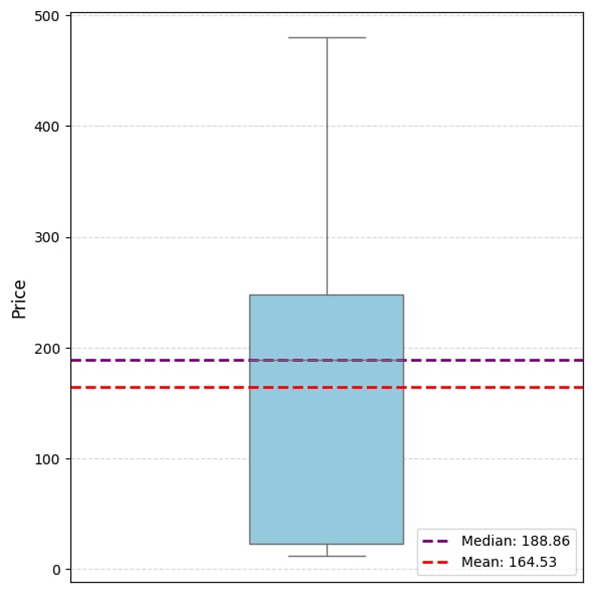
\includegraphics[width=\linewidth]{boxplot.png}
        \caption{TSLA stock price’s boxplot}
        \label{fig:boxplot}
    \end{minipage}
    \hfill
    \begin{minipage}[b]{0.48\linewidth}
        \centering
        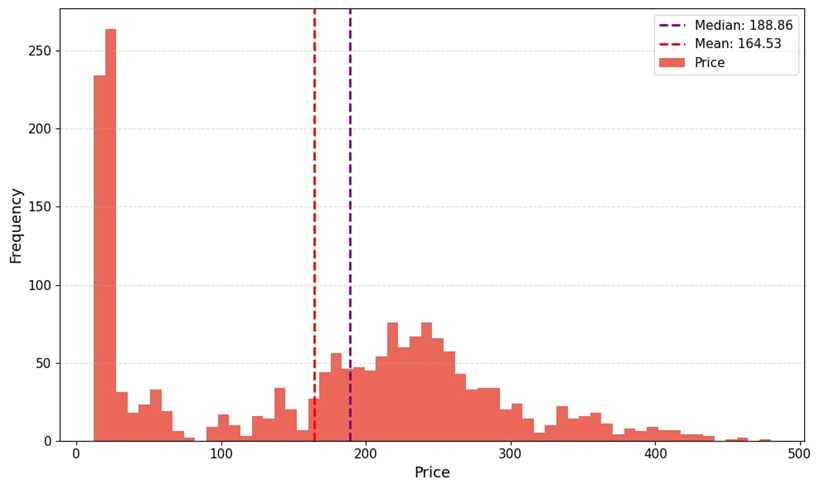
\includegraphics[width=\linewidth]{histogram.png}
        \caption{TSLA stock price’s histogram}
        \label{fig:histogram}
    \end{minipage}
\end{figure}

\begin{table}[H]
    \centering
    \caption{TSLA Descriptive Statistics}
    \label{tab:tsla-stats}
        \begin{tabular}{|c|c|}
        \hline
        \textbf{Descriptive Statistic} & \textbf{TSLA} \\
        \hline
        Count  & 1835 \\
        \hline
        Mean   & 164.525 \\
        \hline
        Std    & 115.339 \\
        \hline
        Min    & 11.931 \\
        \hline
        25\%   & 23.432 \\
        \hline
        50\%   & 188.860 \\
        \hline
        75\%   & 248.197 \\
        \hline
        Max    & 479.860 \\
        \hline
    \end{tabular}
\end{table}


% ==============================================================
% =====================       ARIMA      =======================
% ==============================================================
\section{METHODOLOGY}

\subsection{ARIMA}
ARIMA stands for Autoregressive Integrated Moving Average. The ARIMA model is using three different concepts: autoregressive (AR) model, moving average (MA) model, and integration, together classified as an ARIMA $(p, d, q)$. It is a quantitative forecasting model over time, where the future value of the predictor variable will depend on the movement trend of that object in the past. 
The model contains three components/parameters: AR + I + MA. AR is denoted as $p$, where it shows the weighted linear of sum $p$ values based on ARIMA $(p, d, q)$ terminology. The $p$-value indicates the number of orders. The formula to denote this AR is shown as:

\begin{equation}
\phi_1 = \phi_1 + \phi_2 \delta - \delta x_0 + \phi_3 \delta - \delta x_1 + \ldots + \delta e_{t-1} = e_t
\end{equation}

\noindent Where $p$ is used to determine the number of orders of past values; $t$ is the time series; $\phi$ is the coefficient of the AR model; $e$ is the error term with mean zero and variance $\sigma^2$.

\noindent MA process is denoted by order $q$ in the ARIMA $(p, d, q)$ classification which shows an error value in Equation (4), it also uses the number of orders in the past values, as denoted in equation:
\begin{equation}
y_t = \mu +\theta_1 e_{t-1} + \theta_2 e_{t-2} + \ldots + \theta_q e_{t-q} + e_t
\end{equation}
Where $t$ is the time series; $\theta$ is the slope coefficient; $q$ is the number of orders needed to identify the past values. To identify how many orders are in the calculation of AR, the parameter of $q$ is used; c is the intercept

\noindent Integrated or differentiated versions are denoted as $d$ in ARIMA $(p, d, q)$, which is the number of times the time series got different.

\begin{equation}
I(d) = \Delta(y_t) = y_t - y_{t-1}
\end{equation}
Therefore, The ARIMA(p, d, q) can be represented in the following equation:

\begin{equation}
\small
\begin{array}{l}
y_t = \mu + \phi_0 + \phi_1\Delta(y_{t-1}) + \ldots + \phi_p\Delta( y_{t-p}) \\
\quad +\; \theta_1 \varepsilon_{t-1} + \ldots + \theta_q \varepsilon_{t-q} + \varepsilon_t
\end{array}
\end{equation}


% ==============================================================
% =====================       SVR      =========================
% ==============================================================

\subsection{SVR}
SVR extends Support Vector Machines (SVM) to regression tasks. It aims to find a function:
\begin{align}
    f(x) = \langle w, x \rangle + b
\end{align}
that predicts target values within a margin \(\epsilon\) from the true values, while keeping the function as flat as possible. 
\noindent Primal optimization problem:
\begin{align}
    \min_{w,b,\xi,\xi^*} \quad \frac{1}{2} \|w\|^2 + C \sum_{i=1}^n (\xi_i + \xi_i^*)
\end{align}
Subject to:
\begin{align}
    \begin{cases}
        y_i - \langle w, x_i \rangle - b \leq \epsilon + \xi_i \\
        \langle w, x_i \rangle + b - y_i \leq \epsilon + \xi_i^* \\
        \xi_i, \xi_i^* \geq 0, \quad i=1, \ldots, n
    \end{cases}
\end{align}
Where:
\begin{itemize}
    \item \(\|w\|^2\) controls flatness (regularization).
    \item \(C > 0\) balances model flatness and tolerance for errors greater than \(\epsilon\).
    \item \(\xi_i, \xi_i^*\) are slack variables for deviations outside the \(\epsilon\)-tube.
\end{itemize}
\textbf{Kernel extension (nonlinear SVR):}

\noindent By mapping inputs to a higher-dimensional space using a kernel \(K(x_i, x_j) = \phi(x_i)^T \phi(x_j)\), the prediction becomes:

\begin{align}
    f(x) = \sum_{i=1}^n (\alpha_i - \alpha_i^*) K(x_i, x) + b
\end{align}

% ==============================================================
% =====================       RNN      =========================
% ==============================================================
\subsection{Recurrent Neural Network (RNN)}
A Recurrent Neural Network - RNN is a deep neural network designed to process sequential data such as time series, text, audio,… Unlike traditional feedforward neural networks, RNNs have loops that allow information to persist, making them ideal for tasks where context is crucial.
RNNs process sequential data by maintaining a hidden state that is updated at each time step t, according to the formula:
\begin{align}
h^{(t)} &= g_1\left(W_{xh} x^{(t)} + W_{hh} h^{(t-1)} + b_h\right)
\end{align}
With the output being:
\begin{align}
    y^{(t)} &= g_2\left(W_{hy} h^{(t)} + b_y\right)
\end{align}
Where \( y^{\langle t \rangle} \) is the output at time step \( t \), \( W_x \) is the output weight matrix, and \( b_x \) is the output bias term.

\noindent Where:
\begin{itemize}
    \item \( x^{(t)} \) is the input vector at time step \( t \).
    \item \( y^{(t)} \) is the output vector at time step \( t \), representing the network's prediction.

    \item \( h^{(t-1)} \) is the hidden state from the previous time step, containing information from prior inputs.
    \item \( W_{xh} \), \( W_{hh} \), and \( W_{hy} \) are weight matrices that transform the inputs and hidden states.
    \item \( b_h \) and \( b_y \) are bias vectors.
    \item \( g_1 \) is a nonlinear activation function (e.g., \(\tanh\) or ReLU) applied to compute the hidden state.
    \item \( g_2 \) is an activation function appropriate for the output task (e.g., softmax for classification).
\end{itemize}

% ==============================================================
% =====================       LSTM      ========================
% ==============================================================

\subsection{Long Short-Term Memory (LSTM)}
Long Short-Term Memory (LSTM) is a type of Recurrent Neural Network (RNN) architecture that is capable of learning long-term dependencies in sequence data. Traditional RNNs suffer from the vanishing gradient problem, which limits their ability to capture long-term dependencies. LSTM addresses this issue by introducing memory cells and gated mechanisms.

\begin{figure}[H]
    \centering
    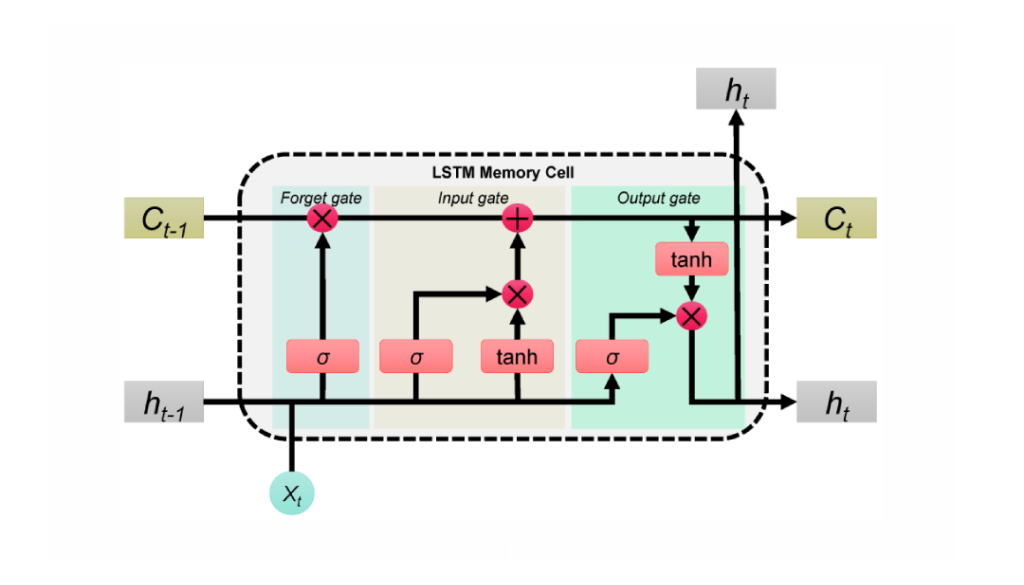
\includegraphics[width=1\linewidth]{LSTM.png}
    \caption{Long Short-Term Memory}
    \label{fig:boxplot}
\end{figure}


\noindent An LSTM cell contains three gates: the input gate, the forget gate, and the output gate. These gates regulate the flow of information and help the network decide what information to keep or discard over time.

\noindent The computations inside an LSTM cell at time step $t$ are defined as follows:

\begin{equation}
f_t = \sigma(W_f x_t + U_f h_{t-1} + b_f)
\end{equation}
\begin{equation}
i_t = \sigma(W_i x_t + U_i h_{t-1} + b_i)
\end{equation}
\begin{equation}
\tilde{c}_t = \tanh(W_c x_t + U_c h_{t-1} + b_c)
\end{equation}
\begin{equation}
c_t = f_t \odot c_{t-1} + i_t \odot \tilde{c}_t
\end{equation}
\begin{equation}
o_t = \sigma(W_o x_t + U_o h_{t-1} + b_o)
\end{equation}
\begin{equation}
h_t = o_t \odot \tanh(c_t)
\end{equation}

\noindent Where:
\begin{itemize}
    \item $x_t$ is the input at time $t$
    \item $h_{t-1}$ is the hidden state from the previous time step
    \item $f_t$, $i_t$, and $o_t$ are the forget, input, and output gates respectively
    \item $c_t$ is the cell state at time $t$, and $\tilde{c}_t$ is the candidate value for the cell state
    \item $W_*$, $U_*$, $b_*$ are weight matrices and bias vectors
    \item $\sigma$ is the sigmoid activation function
    \item $\tanh$ is the hyperbolic tangent function
    \item $\odot$ denotes element-wise multiplication
\end{itemize}

\noindent LSTM is particularly well-suited for time-series forecasting tasks such as stock price prediction, as it can capture both short-term fluctuations and long-term trends in sequential data.


% ==============================================================
% =====================       RESNET      ======================
% ==============================================================
\subsection{Residual Network (ResNet)}\label{sec:intro}
ResNet (or residual network) is a type of deep neural network that is able to perform very well, of with the vanishing gradient as depths grows. It applies residual blocks that have 3 convolutional blocks using different kernel size through shortcut connection that adds initial input to a block output. The ResNet as described in this work consists of three blocks and then is connected to a global average pooling layer and a fully connected layer for the final output.

% Describing the residual block and equations
\subsubsection{Residual Block}
Each residual block uses 1 x 1 convolutions to create three convolutional blocks which are set up as follows:
\begin{align}
h_1 &= \text{ReLU}(\text{BN}(\text{Conv1d}(x))), \label{eq:h1} \\
h_2 &= \text{ReLU}(\text{BN}(\text{Conv1d}(h_1))), \label{eq:h2} \\
h_3 &= \text{BN}(\text{Conv1d}(h_2)). \label{eq:h3}
\end{align}
After computing \(h3\), the value is relayed to a linear unit. Output of the residual block is then calculated by \(x\) plus relaying \(h3\) while applying the relayed value on a linear unit:
\begin{align}
y &= h_3 + x, \label{eq:y} \\
\hat{h} &= \text{ReLU}(y). \label{eq:hhat}
\end{align}
The convolutional blocks use kernel sizes of 7, 5 and 3. The three residual blocks will have the filter count set to \( k_i = \{64, 128, 128\} \).

% ==============================================================
% ================       RESNET-LSTM      ======================
% ==============================================================
\subsection{ResNetLSTM Model}
The architecture of ResNet-LSTM includes ResNet for spatial feature extraction and LSTM for time-series modeling. We adopt ResNet based on ResNet18 to extract features by convolution processes along with residual blocks, which provide a feature tensor as input to the LSTM. The LSTM component incorporates temporal dependencies using 2 layers with 1024 and 256 units each. They utilized dropout to prevent overfitting as well as 2 dense layers for prediction which consisted of 64 and 1 neurons respectively.[1]. In the implemented model, an LSTM layer with 50 units is added to process the transposed ResNet output:
\begin{equation}
x_{\text{lstm}} = x.\text{transpose}(1, 2), \label{eq:transpose}
\end{equation}
Followed by:
\begin{equation}
x_{\text{lstm}}, (h_n, c_n) = \text{LSTM}(x_{\text{lstm}}). \label{eq:lstm}
\end{equation}
The final time step output is selected:
\begin{equation}
x_{\text{final}} = x_{\text{lstm}}[:, -1, :]. \label{eq:final}
\end{equation}
The prediction is produced through the application of a fully connected (FC) layer:
\begin{equation}
y = \text{FC}(x_{\text{final}}). \label{eq:output}
\end{equation}


% ==============================================================
% ============       EXPERIMENTAL RESULTS     ==================
% ==============================================================
\section{EXPERIMENT RESULT}

The evaluation metrics are calculated by measuring errors, such as Mean Absolute Error (MAE), Mean Absolute Percentage Error (MAPE), Mean Absolute Scaled Error (MASE), Mean Squared Error (MSE), and Root of Mean Squared Error (RMSE,).
\[
\text{MAE} = \frac{1}{n} \sum_{i=1}^n |y_i - \hat{y}_i|
\]
\[
\text{MAPE} = \frac{1}{n} \sum_{i=1}^n \left| \frac{y_i - \hat{y}_i}{y_i} \right| \times 100
\]
\[
\text{MASE} = \frac{1}{n} \sum_{i=1}^n \frac{|y_i - \hat{y}_i|}{\frac{1}{m-1} \sum_{j=1}^{m-1} |y_{j+1}^{\text{train}} - y_j^{\text{train}}|}
\]
\[
\text{MSE} = \frac{1}{n} \sum_{i=1}^n (y_i - \hat{y}_i)^2
\]
\[
\text{RMSE} = \sqrt{\frac{1}{n} \sum_{i=1}^n (y_i - \hat{y}_i)^2}
\]
where \( y_i \) is the actual price, \( \hat{y}_i \) is the predicted price, \( n \) is the number of predictions, and \( y^{\text{train}} \) is the training data.

% ==============================================================
% ARIMA
\subsection{ARIMA}
Input Layer: Univariate time series data — Close price of TSLA stock.
\noindent Model Order: ARIMA(3,1,2) — determined through auto arima optimization.
\noindent Parameters:
\begin{itemize}
\item p = 3 — autoregressive terms
\item d = 1 — differencing order
\item q = 2 — moving average terms
\end{itemize}
\noindent Data Preprocessing:
\begin{itemize}
\item Logarithmic transformation
\item First-order differencing for stationarity
\item ADF test for stationarity verification
\end{itemize}

\begin{figure}[H]
    \centering
    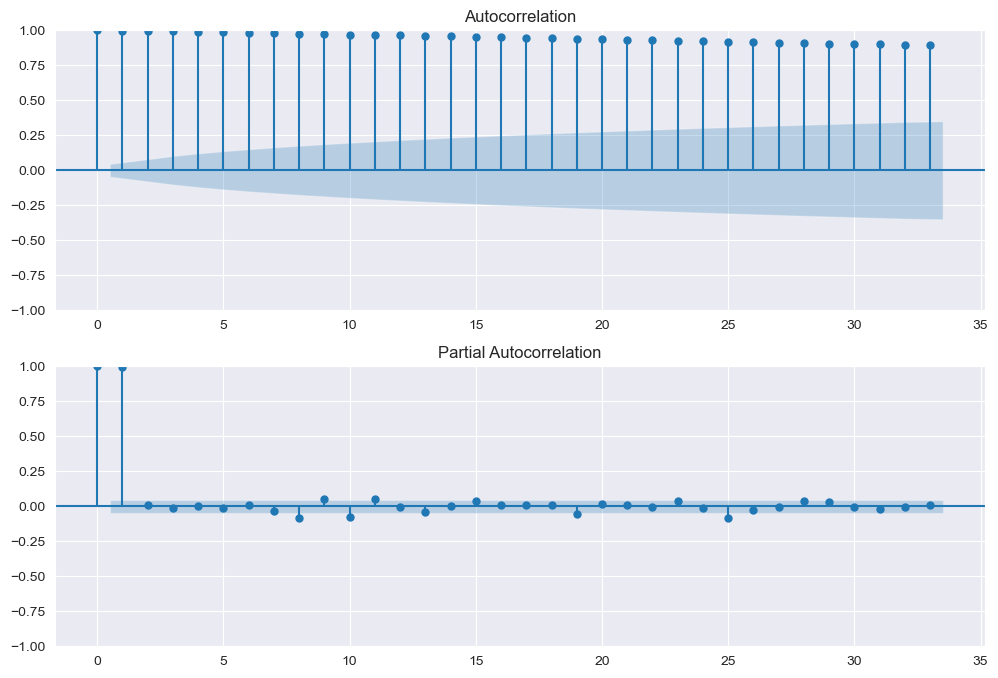
\includegraphics[width=1\linewidth]{Autocorrelation.png}
    \caption{Autocorrelation}
    \label{fig:boxplot}
\end{figure}

\noindent Training Process:
\begin{itemize}
\item Train-test split: 80-20 ratio
\item Auto ARIMA for parameter optimization
\item AIC criterion for model selection
\end{itemize}
\noindent Model Evaluation: Mean Squared Error (MSE) for regression performance.

\begin{figure}[H]
    \centering
    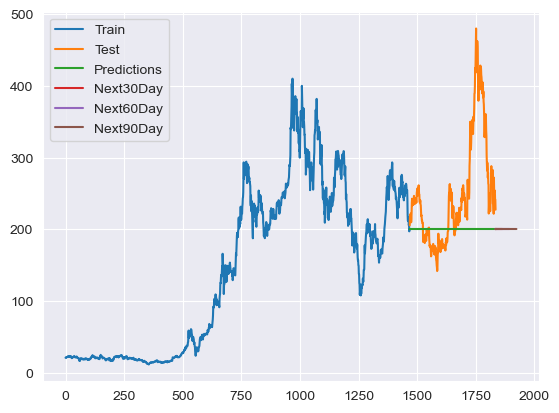
\includegraphics[width=1\linewidth]{Arima.png}
    \caption{ARIMA TSLA 8-2 }
    \label{fig:boxplot}
\end{figure}

% ==============================================================
% LSTM
\subsection{LSTM}
Input Layer: Input shape: $(100, 1)$ — univariate time series with time steps $= 100$.
\noindent LSTM Layers:
\begin{itemize}
\item First LSTM Layer: 50 units with return sequences=True
\item Second LSTM Layer: 50 units with return sequences=True
\item Third LSTM Layer: 50 units
\end{itemize}
\noindent Dense Layer (Output Layer): 1 neuron — linear activation for regression output.
\noindent Data Preprocessing:
\begin{itemize}
\item MinMaxScaler: feature range=(0,1)
\item Train-test split: 80-20 ratio
\item Sequence creation with time step=100
\end{itemize}
\noindent Training Parameters:
\begin{itemize}
\item Loss function: Mean Squared Error (MSE)
\item Optimizer: Adam
\item Epochs: 100
\item Batch size: 64
\item Validation data: 20\% of dataset
\end{itemize}
\noindent Model Evaluation: RMSE, MAPE, and MAE metrics for performance assessment.

\begin{figure}[H]
    \centering
    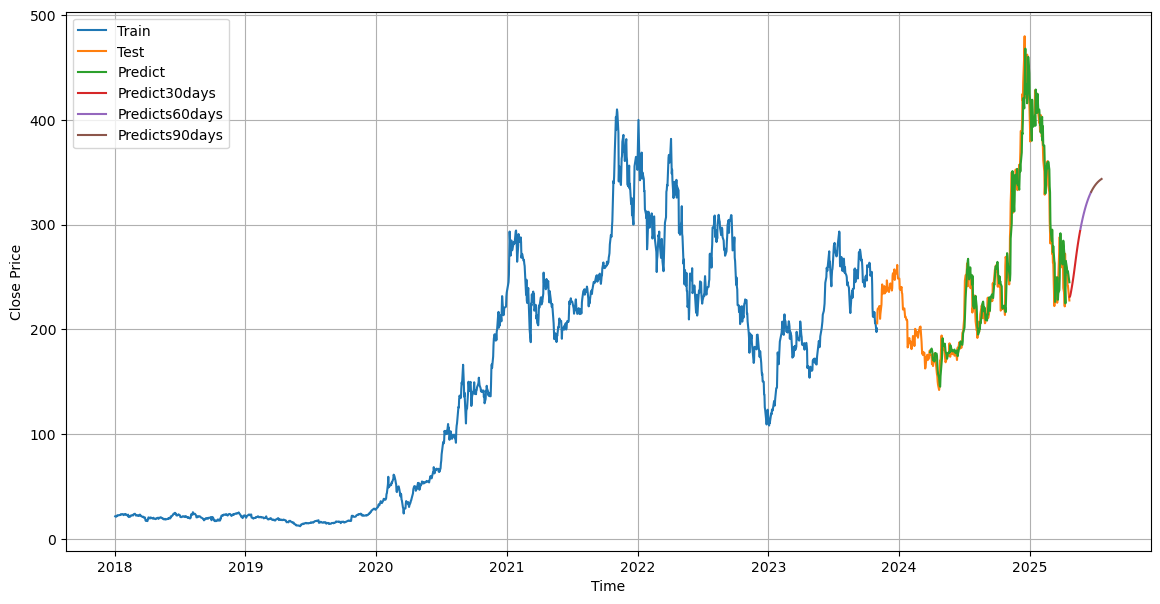
\includegraphics[width=1\linewidth]{LSTM_8_2.png}
    \caption{LSTM TSLA 8-2 }
    \label{fig:boxplot}
\end{figure}


% ==============================================================
% SVR
\subsection{SVR}

\begin{itemize}
    \item SVR with Linear Kernel: \texttt{kernel= linear}, \( C = 100 \)
    \item SVR with RBF Kernel:
    \begin{itemize}
        \item Configuration 1: \( C = 100 \), \( \epsilon = 0.0001 \), \( \gamma = 10 \)
        \item Configuration 2: \( C = 1{,}500{,}000 \), \( \epsilon = 10^{-7} \), \( \gamma = 100 \)
    \end{itemize}
    \item SVR with Polynomial Kernel: \texttt{kernel= poly }, \( C = 100 \), \( \epsilon = 0.0001 \), degree = 3
\end{itemize}
\begin{table}[H]
    \centering
    \caption{RMSE results of SVR models with different kernels}
    \label{tab:svr_results}
    \begin{tabular}{|l|c|}
        \hline
        \multicolumn{1}{|c|}{\textbf{Model}} & \textbf{RMSE} \\
        \hline
        SVR Linear & 0.6342 \\
        SVR RBF (C=100, $\epsilon$=0.0001, $\gamma$=10) & 0.2061 \\
        \textbf{SVR RBF (C=1,500,000, $\epsilon$=1e-7, $\gamma$=100)} & \textbf{0.1306} \\
        SVR Polynomial & 0.7265 \\
        \hline
    \end{tabular}
\end{table}

\begin{figure}[H]
    \centering
    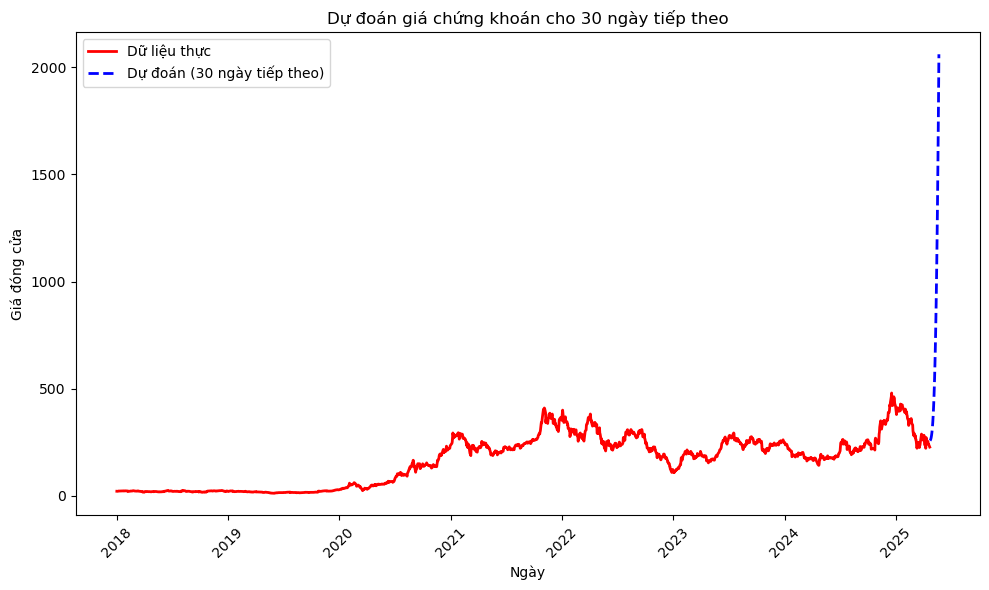
\includegraphics[width=1\linewidth]{SVR.png}
    \caption{SVR TSLA 8-2 }
    \label{fig:boxplot}
\end{figure}

% ==============================================================
% RNN
\subsection{RNN}

Input Layer: Input shape: $(100, 1)$ — univariate time series with time\_steps $= 100$.

\noindent SimpleRNN Layer: 50 units — basic RNN for sequential data processing.

\noindent Dense Layer (Output Layer): 1 neuron — linear activation for regression output.

\noindent Loss function: Mean Squared Error (MSE) — suitable for regression tasks.

\noindent Optimizer: Adam — adaptive learning rate.

\noindent Epochs: 24 — full passes over the training data.

\noindent Batch size: 64 — samples per gradient update.

\noindent Verbose: 1 — show training progress.

\begin{figure}[H]
    \centering
    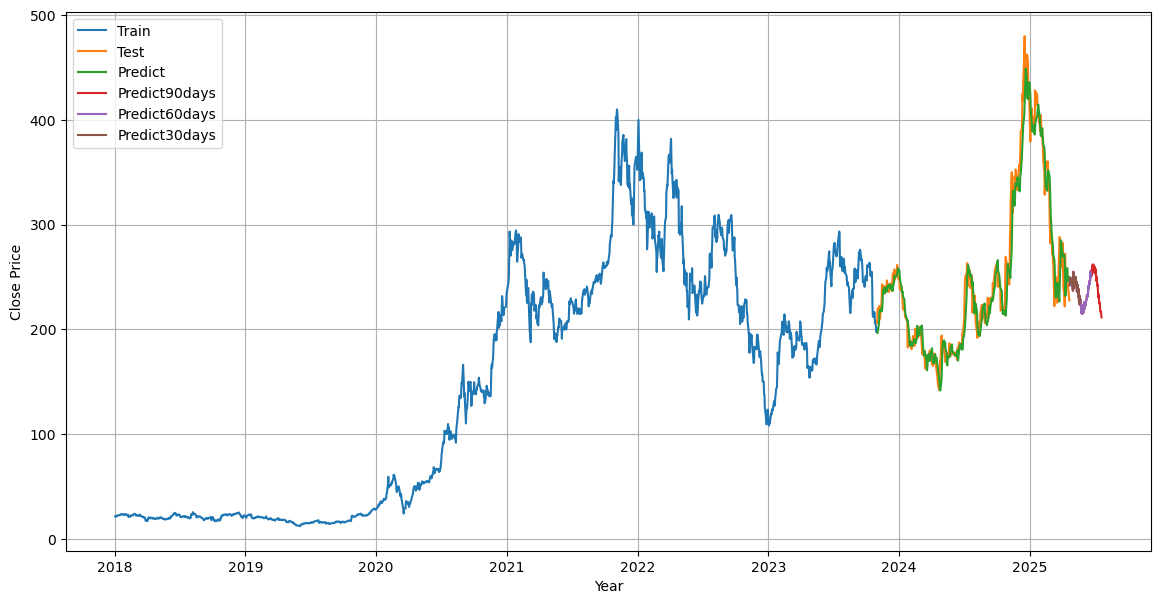
\includegraphics[width=1\linewidth]{RNN.png}
    \caption{RNN TSLA 8-2 }
    \label{fig:boxplot}
\end{figure}

% ==============================================================
% ResNet
\subsection{ResNet}
The design layout of the ResNet model is as follows:

\begin{equation}
\begin{aligned}
\text{ResNet} = [&\text{ResBlock1}, \text{ResBlock2}, \\
                &\text{ResBlock3}, \text{GlobalAvgPooling}, \text{FC}].
\end{aligned}
\end{equation}


\noindent The model receives input data and computes it through the three residual blocks, then bounds global average pooling to spatial dimensionality reduction, then ultimately produces the output through a fully connected layer detached from the pooling operation.

\begin{figure}[H]
    \centering
    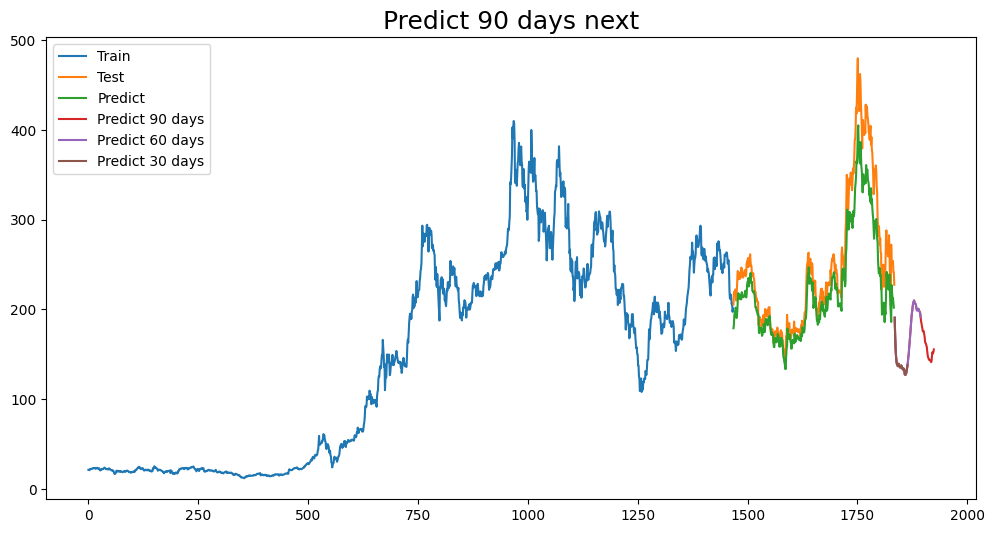
\includegraphics[width=1\linewidth]{resnet_predictions.png}
    \caption{ResNet TSLA 8-2 }
    \label{fig:boxplot}
\end{figure}

% ==============================================================
% ResNetLSTM
\subsection{ResNetLSTM}
The total architecture is:

\begin{equation}
\begin{aligned}
\text{ResNetLSTM} = [&\text{ResBlock1}, \text{ResBlock2}, \\
                     &\text{ResBlock3}, \text{LSTM}, \text{FC}].
\end{aligned}
\end{equation}

\noindent Model training was done using the Adam optimizer with a learning rate set at 0.001, mean squared error (MSE) loss, a batch size of 64, and 100 epochs.

\begin{figure}[H]
    \centering
    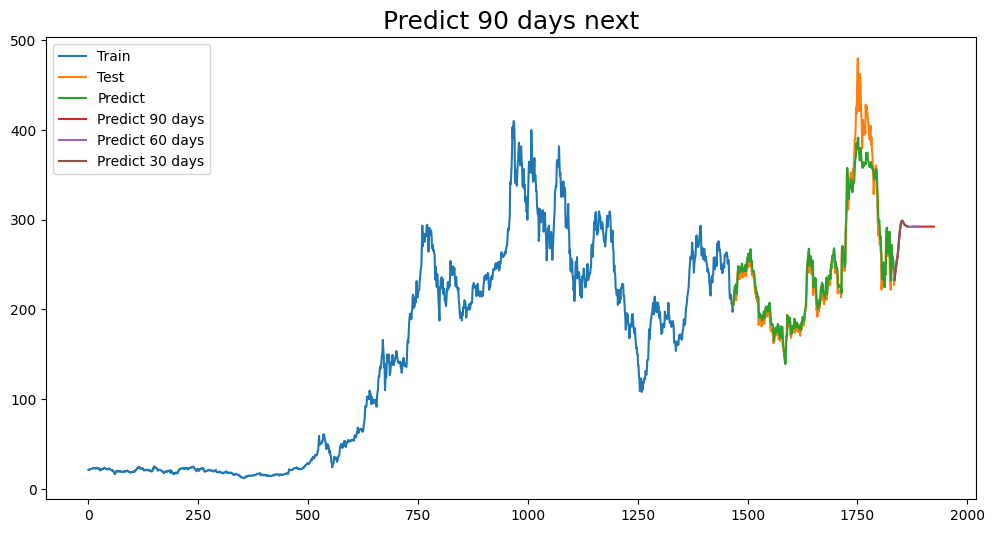
\includegraphics[width=1\linewidth]{resnetlstm_predictions.png}
    \caption{ResNetLSTM TSLA 8-2 }
    \label{fig:boxplot}
\end{figure}

\noindent The results are summarized in Table~\ref{tab:results}.
\begin{table}[H]
\centering
\caption{Forecasting performance of ResNet and ResNetLSTM on the test set.}
\label{tab:results}
\resizebox{\columnwidth}{!}{%
\begin{tabular}{lccccc}
\toprule
Model & MAE & MAPE (\%) & MASE & MSE & RMSE \\
\midrule
ResNet & 24.8383 & 8.7462 & 2651.4954 & 1253.6210 & 35.4065 \\
ResNetLSTM & 23.3139 & 7.7512 & 2488.7656 & 1254.4014 & 35.4175 \\
\bottomrule
\end{tabular}
}
\end{table}

\subsection{Evaluation Results}
\vspace{-2em}

\begin{table}[H]
\centering
\caption{Comparison of forecasting performance across models}
\label{tab:model_comparison}
\resizebox{\columnwidth}{!}{%
\begin{tabular}{lcc}
\toprule
Model & MAE & RMSE \\
\midrule
ARIMA & 61.109 & 88.889 \\
RNN & 9.620 & 13.800 \\
LSTM & 263.064 & 275.176 \\
GRU & 251.373 & 261.875 \\
ResNet & 25.420 & 32.440 \\
ResNet-LSTM & 12.553 & 19.304 \\
\bottomrule
\end{tabular}
}
\end{table}

\section{CONCLUSION}
This study conducted a comparative analysis of various machine learning and deep learning models for forecasting Tesla's stock prices using historical time-series data. The evaluation metrics, specifically MAE and RMSE, clearly demonstrate the variability in performance across different models. Traditional statistical models like ARIMA showed the weakest performance, with the highest MAE (61.109) and RMSE (88.889), indicating limited capability in capturing the nonlinear patterns in stock data. 

\noindent Among deep learning models, ResNet-LSTM achieved the lowest error metrics (MAE: 12.553, RMSE: 19.304), suggesting its superior ability to model both spatial and temporal dependencies. The standalone RNN model also performed well (MAE: 9.620, RMSE: 13.800), surpassing the more complex LSTM and GRU models, which were affected by higher error values. Notably, LSTM and GRU underperformed, with RMSE values above 260, highlighting their limitations in this context.

Overall, the hybrid ResNet-LSTM model emerged as the most effective approach for Tesla stock prediction, balancing both residual feature extraction and sequence learning. 





% ---- Bibliography ----

\begin{thebibliography}{8}
\bibitem{ref_article1}
\href{https://www.kaggle.com/code/guslovesmath/tesla-stock-forecasting-multi-step-stacked-lstm}{Kaggle code for lsmt tesla stock forecasting}

\bibitem{ref_lncs1}
\href{https://www.researchgate.net/publication/373013410_Stock_Price_Prediction_of_Tesla_Apple_using_LSTM}{Stock Price Prediction of Tesla, Apple using LSTM}, ResearchGate, 2023.


\bibitem{ref_lncs1}
\href{https://github.com/JinleiZhangBJTU/ResNet-LSTM-GCN}{Stock Price Prediction, Apple using ResNetLSTM}, ResearchGate, 2023.

\bibitem{ref_long2025}
Duong Phi Long, ``Lecture Notes'' University of Information Technology. Unpublished lecture material


\end{thebibliography}
\end{document}
